\documentclass[twocolumn, natbib]{svjour3}
\usepackage{graphicx}%GRaphiken
\usepackage[utf8]{inputenc}
\usepackage{tabularx}%Tabellen!
\usepackage[english]{babel}
\usepackage{textcomp}% Sonderzeichen
\usepackage{amsmath}%maths / equations
\usepackage{mathptmx}
\usepackage{url}
\usepackage{marvosym}
\newcommand{\envelope}{(\raisebox{-.5pt}{\scalebox{1.45}{\Letter}}\kern-.1pt) }

% to compare to old
% cd /home/edisz/Documents/Uni/Projects/PHD/6USETHEGLM/manuscript/
% % first compare bibliography
% latexdiff submission/report/report.bbl revision/report/report.bbl > revision/diff/diff.bbl

% % then document
% latexdiff --disable-citation-markup --math-markup=3 --append-context2cmd=subtitle submission/report/report.tex revision/report/report.tex > revision/diff/diff.tex



%% ----------------------------------------------------------------------------
\title{Ecotoxicology is not normal.}
\subtitle{A comparison of statistical approaches for analysis of count and proportion data in ecotoxicology.}
\author{Eduard Szöcs \and Ralf B. Schäfer}
\institute{Eduard Szöcs \envelope  and Ralf B. Schäfer \at
Institute for Environmental Sciences \\
University Koblenz-Landau \\
Fortstraße 7, \\
76829 Landau, Germany \\
Tel.: +49 06341 280 31552 \\
\email{szoecs@uni-landau.de}
}
\date{Received: date / Accepted: date}
\journalname{Environmental Science and Pollution Research}



%% ----------------------------------------------------------------------------
\begin{document}
\sloppy
\maketitle

%% ----------------------------------------------------------------------------
\begin{abstract}
Counts and proportions are data types often encountered by ecotoxicologists, which are rarely normally distributed.
To meet the assumptions of normality and heteroscedasticity, the standard procedure has been to either transform the data or use non-parametric methods if this fails.
Generalised Linear Models (GLM) allow directly model distributions fitting such data.
Here, we compare the performance of parametric methods assuming (1) normality of transformed data, (2) appropriate distributions (Poisson, negativ binomial, binomial) and (3) non-parametric methods.

We simulated typical data mimicking low replicated ecotoxicological experiments of two common data types (counts and proportions from counts). 
We compared the performance of different methods in terms of statistical power and type 1 error for detecting a general treatment effect and determining the lowest observed effect concentration (LOEC).
In addition, we outlined differences and advantages of GLMs on a real world mesocosm data set.

For counts, we found that the quasi-Poisson model and the negative binomial model in combination with the parametric boostrap had higher statistical power than data transformation.
For proportions GLMs performed better, except to determine LOEC at extremly low sample sizes.
The compared non-parametric methods had generally lower power.

We recommend that counts and proportions from counts should be analysed by making appropriate distributional assumptions and GLMs should become a standard method in ecotoxicology.
 \keywords{Generalized Linear Models \and Transformations \and Simulation \and Power \and Type 1 error}
\end{abstract}



%% ----------------------------------------------------------------------------
\section{Introduction}
\label{sec:intro}
Ecotoxicologists perform various kinds of experiments yielding different types of data.
Examples are animal counts in mesocosm experiments (non-negative, integer-valued data) or proportions of surviving animals (data bounded between 0 and 1, discrete).
These data are typically not normally distributed. 
Nevertheless, they are often analysed using methods assuming a normal distribution and variance homogeneity \citep{wang_making_2011}. 
To meet these assumptions, data are usually transformed.
For example, ecotoxicological textbooks \citep{newman_quantitative_2012} and guidelines \citep{epa_methods_2002,oecd_current_2006} advise that survival data can be transformed using an arcsine square root transformation. 
For count data from mesocosm experiments a log(Ay + C) transformation is usually applied, where the constants A and C are either chosen arbitrarily or following general recommendations. 
For example, \citet{van_den_brink_impact_2000} suggest to set the term Ay to be 2 for the lowest abundance value (y) greater than zero and C to 1. 
Moreover, other transformations like the square root or fourth root are commonly applied in community ecology.
Note that there has been little evaluation and advice for practitioners, which transformations to use.
If the transformed data still do not meet the assumptions (i.e. normality and variance homogeneity), non-parametric tests are usually applied \citep{wang_making_2011}.

Generalised linear models (GLM) provide a method to analyse counts or proportions from counts in a  statistically sound way \citep{nelder_generalized_1972}.
GLMs can handle various types of data distributions, e.g. Poisson or negative binomial (for count data) or binomial (for proportions); the normal distribution being a special case of GLMs.
Despite GLMs being available more than 40 years, ecotoxicologists do not regularly make use of them.
Recent studies concluded that data transformations should be avoided and GLMs be used as they have better statistical properties (\citealt{ohara_not_2010} (counts), \citealt{warton_arcsine_2011,warton_many_2005} (proportions from counts)). 

Ecotoxicological experiments often involve small sample sizes due to practical constraints. 
For example, extremely low samples sizes (n \textless 5) are common in many mesocosm studies \citep{sanderson_pesticide_2002,szocs_analysing_2015}.
Small sample sizes lead to low power in statistical hypothesis testing, on which many ecotoxiological approaches (e.g. risk assessment for pesticides) rely. 
Such an endpoint are L/NOEC (Lowest / No observed effect concentration) values.
Although their use has been heavily criticized in the past \citep{laskowski_good_1995}, they are the predominant endpoint in mesocosm experiments \citep{brock_minimum_2015, efsa_ppr_guidance_2013}. 

We explore how GLMs may enhance inference in ecotoxicological studies and compared three types of statistical methods (transformation and normality assumption, GLM, non-parametric tests).
We first illustrate differences between statistical methods using a data set from a mesocosm study.
Then we further elaborate differences in detecting a general treatment effect and determining the LOEC using simulations of two common data types in ecotoxicology: counts and proportions from counts. 



%% ----------------------------------------------------------------------------
\section{Methods}
\label{sec:methods}

%% --------------------------------
\subsection{Models for count data}
\label{ssec:counts}
\subsubsection{Linear model for transformed data}
To meet the assumptions of the standard linear model, count data usually needs to be transformed. 
We followed the recommendations of \citet{van_den_brink_impact_2000} and used a log(Ay + 1) transformation (eqn. \ref{eqn:trans}):
\begin{align}
  y_i^T & = log(Ay_i + 1) \label{eqn:trans}
\end{align}

, where $y_i$ is the measured and $y_i^T$ the transformed abundance of the $i$th observation. 
The factor $A$ was chosen in such way that $Ay$ equals 2 for the lowest non-zero abundance value (y).

Then we fitted the linear model to the transformed abundances (hereafter $LM$):
\begin{align}
  y_i^T &\sim N(\mu_i, \sigma^2) \nonumber \\
  E(y_i^T) = \mu_i ~&\text{and}~ var(y_i^T) = \sigma^2 \label{eqn:normal} \\
  \mu_i &= \beta Treatment_i  \nonumber
\end{align}

This model assumes a normal distribution of the transformed abundances.
The expected value for each observation $i$ is given by its mean ($\mu_i$) and the variance ($\sigma^2$) is constant between treatments.
We allow this mean to vary between treatments and $\beta$ are the coefficients related to these changes in transformed abundances between treatments (eqn. \ref{eqn:normal}).


\subsubsection{Generalised Linear Models}
GLMs extend the normal model by modelling other distributions.
Instead of transforming the response variable, the counts could be directly modelled by a Poisson GLM ($GLM_p$):
\begin{align}
  y_i &\sim P(\mu_i) \nonumber \\
  E(y_i) &= var(y_i) = \mu_i \label{eqn:pois} \\
  log(\mu_i) &= \beta Treatment_i  \nonumber
\end{align}

This model assumes poisson distributed abundances with mean $\mu_i \ge 0$.
The expected value for each observation $i$ is given by its mean. 
Moreover, this model assumes that mean and variance are equal.
We are modelling the mean as a function of treatment membership.
However, to avoid negative values of the mean this is done on a log scale.
Therefore, $\beta$ also describes the differences between treatments on a log scale (eqn. \ref{eqn:pois}).

The assumption of equal mean and variance is rarely met with ecological data, which is typically characterized by greater variance than the mean (overdispersion).
To overcome this problem a quasi-Poisson model ($GLM_{qp}$) could be used, which assumes that variance is a linear function of the mean (eqn. \ref{eqn:quasi}):
\begin{align}
  var(y_i) &= \Theta \mu_i  \label{eqn:quasi}
\end{align}

Here, $\Theta$ is used to account for additional variation and is known as overdispersion parameter.
The quasi-Poisson model is a post hoc method, meaning that first a Poisson model is estimated (eqn. \ref{eqn:pois}) and than the standard errors are scaled by the degree of overdispersion.

Another possibility to deal with overdispersion is to fit a negative binomial distribution ($GLM_{nb}$, eqn. \ref{eqn:negbin}):
\begin{align}
  y_i &\sim NB(\mu_i, \kappa) \nonumber  \\
  E(y_i) = \mu_i ~&\text{and}~var(y_i) = \mu_i + \mu_i^2 / \kappa \label{eqn:negbin} \\
  log(\mu_i) &= \beta Treatment_i  \nonumber 
\end{align}

This models assumes that abundances are negative binomially distributed, with a mean of $\mu_i \ge 0$ and a variance $\mu_i + \mu_i^2 / \kappa$.
Similar to the Poisson model we use a log link between mean and treatments.
Note, that the quasi-Poisson model assumes a linear mean-variance relationship (eqn. \ref{eqn:quasi}), whereas the negative binomial model assumes a quadratic relationship (eqn. \ref{eqn:negbin}).

The above described models are most commonly used in ecology \citep{ver_hoef_quasi-poisson_2007}, although other distributions for count data are possible, like the negative binomial model with a linear mean-variance relationship (also known as NB1) or the poisson inverse gaussian model \citep{hilbe_modeling_2014}.


\subsection{Models for binomial data}
\label{ssec:bin}
A binomial variable counts how often an event $x$ occurs in a fixed number of independent trials $N$ (e.g. \emph{"5 out of 10 fish survived"}), with an equal probability of occurrence $\pi$ between trials.
The number of times an event occurs can also be calculated as proportion $x / N$.

\subsubsection{Linear model for transformed data}
To accommodate the assumptions for the standard linear model with such proportions, a special arcsine square root transformation (eqn. \ref{eqn:arcsine}) is suggested \citep{epa_methods_2002,newman_quantitative_2012}:
\begin{align}
  y_i^T = 
  \begin{cases}  
    arcsin(1) - arcsin(\sqrt{\frac{1}{4n}}) & \text{, if}\ y_i = 1 \\
    arcsin(\sqrt{\frac{1}{4n}}) & \text{, if}\ y_i = 0  \\
    arcsin(\sqrt{y_i}) & \text{, otherwise}
  \end{cases} \label{eqn:arcsine}
\end{align}

, where $y_i^T$ are the transformed proportions and n is the total number of exposed animals per treatment.
The transformed proportions are then analysed using the standard linear model ($LM$, eqn. \ref{eqn:normal}).
Note, that the parameters of the linear model are not directly interpretable due to transformation.


\subsubsection{Generalised Linear Models}
A more natural way to model such data is the  binomial distribution with parameters N and $\pi$ ($GLM_{bin})$:
\begin{align}
  y_i &\sim Bin(N, \pi_i) \nonumber \\
  E(y_i) = \pi_i \times N ~&\text{and}~var(y_i) =  \pi_i (1 - \pi_i) / N \label{eqn:bin} \\
  logit~(\pi_i) &= \beta Treatment_i \nonumber
  \end{align}

This model assumes that the number of occurences are binomially distributed, where N = number of trials (e.g. exposed animals) and $\pi_i$ is the probability of occurrences (fish survived), which together give the expected number of occurrences.
The variance of the binomial distribution is a quadratic function of the mean.
We are modelling the probability of occurrence as function of treatment membership and to ensure that $0 < \pi_i < 1$ we do this on a logit scale (eqn. \ref{eqn:bin}). 
However, the parameters $\beta$ of this model are directly interpretable as changes in log odds between treatments.

Similarly to counts, binomial data may also show overdispersion. 
Methods to deal with overdispersed binomial data are either quasi methods (see above) or Generalized Linear Mixed models (GLMM).
However, these are not further investigated in this paper (see \citet{warton_arcsine_2011} for a comparison).


%% --------------------------------
\subsection{Statistical Inference}
After model fitting and parameter estimation the next step is statistical inference.
Ecotoxicologists are generally interested in two hypotheses: (i) is there any treatment related effect? and (ii) which treatments show a treatment effect (to determine the LOEC)?

Following general recommendations \citep{bolker_generalized_2009,faraway_extending_2006}, we used F-tests ($LM$ and $GLM_{qp}$) and Likeli\-hood-Ratio (LR) tests ($GLM_p$, $GLM_{nb}$ and $GLM_{bin}$) to test the first hypothesis.
However, it is well known that LR test are unreliable with small sample sizes \citep{wilks_large-sample_1938}.
Therefore, we additionally explored the parametric bootstrap \citep{faraway_extending_2006} to assess the significance of the LR.
Bootstrapping is computationally very intensive and for this reason we applied it only for the negative binomial models (using 500 bootstrap samples, denoted as $GLM_{npb}$).

To assess the LOEC we used Dunnett contrasts \citep{dunnett_multiple_1955} with one-sided Wald t tests (normal and quasi-Poisson models) and one-sided Wald Z tests (Poisson, negative binomial and binomial models).
Beside these parametric methods we also applied two, in ecotoxicology commonly used, non-parametric methods: The Kruskal-Wallis test  ($KW$) to test for a general treatment effect and a pairwise Wilcoxon test ($WT$) to determine the LOEC.
We adjusted for multiple testing using the method of \citet{holm_simple_1979}.



%% --------------------------------
\subsection{Case study}
\citet{brock_minimum_2015} presents a typical example of data from mesocosm studies, which we use to demonstrate differences between methods.
The data are mayfly larvae counts on artificial substrate samplers were at one sampling date. 
A total of 18 mesocosm have been sampled from 6 treatments (Control (n = 4), 0.1, 0.3, 1, 3 mg/L (n = 3) and 10 mg/L (n = 2)) (Figure \ref{fig:example}).

\begin{figure}[h]
  \centering
  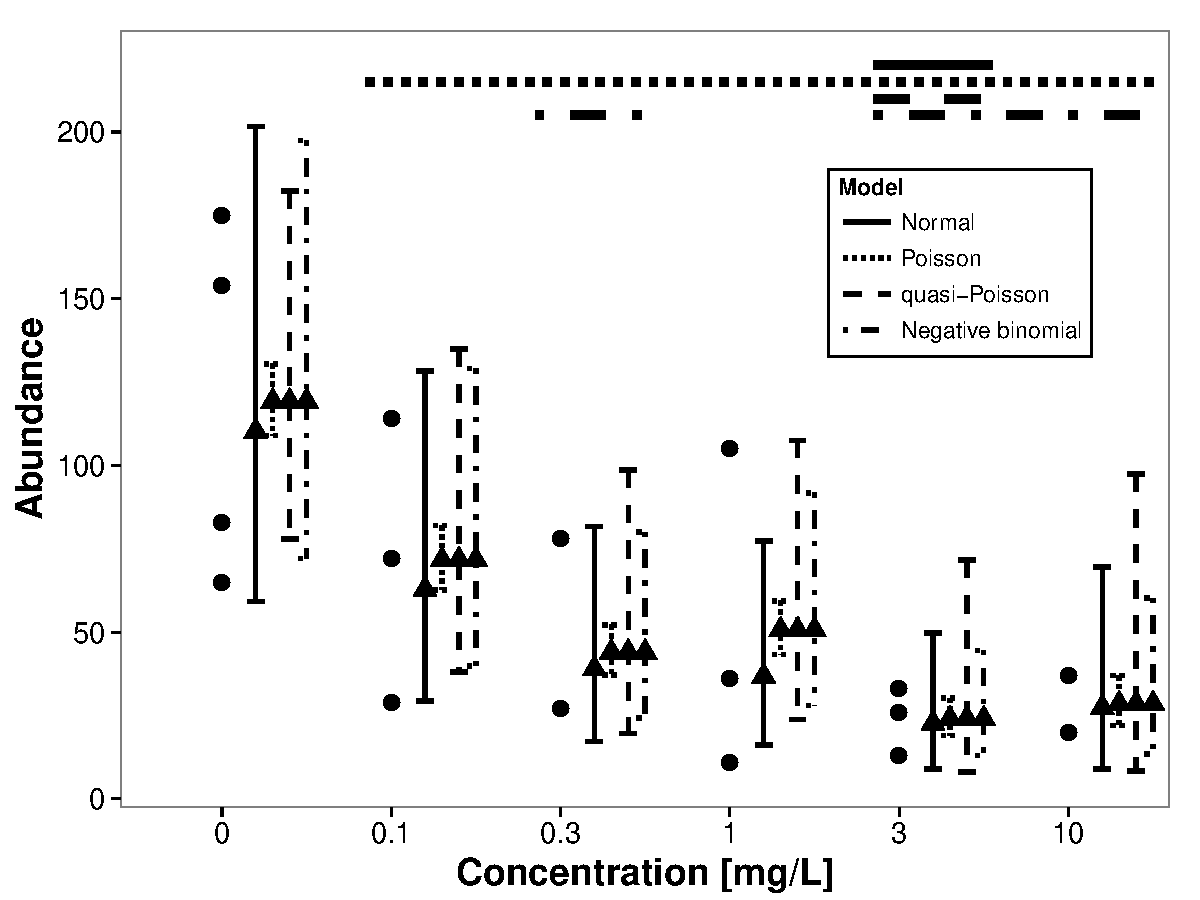
\includegraphics[width = 84mm]{example.pdf}
  \caption{Data from \citet{brock_minimum_2015} (dots). 
  Predicted values (triangles) and 95\% Wald Z or t confidence intervals from the fitted models (vertical lines) are given beside.
  Horizontal bars above indicate treatments statistically significant different from the control group (Dunnett contrasts).
  The data showed overdispersion ($\kappa = 4$) and therefore, the Poisson model underestimates the width of confidence intervals.
  }
  \label{fig:example}
\end{figure}


%% --------------------------------
\subsection{Simulations}
\subsubsection{Count data}
To further scrutinise the differences between methods we simulated data sets with known properties.
We simulated count data that mimics the data of the case study with five treatments (T1 - T5) and one control group (C).
Counts were drawn from a negative binomial distribution with overdispersion at all treatments ($\kappa = 4$, eqn. \ref{eqn:negbin}).
We simulated data sets with different number of replicates (N = \{3, 6, 9\}) and different abundances in control treatments ($\mu_\text{\tiny C}$ = \{2, 4, 8, 16, 32, 64, 128\}). 
For power estimation, mean abundance in treatments T2 - T5 was reduced to half of control and T1 ($\mu_\text{\tiny T2}~=~...~=~\mu_\text{\tiny T5}~=~0.5~\mu_\text{\tiny C} = 0.5~\mu_\text{\tiny T1}$), resulting in a theoretical LOEC at T2.
Mean abundance was kept equal between all groups in Type 1 error simulations.
We generated 1000 data sets for each combination of N and $\mu_\text{\tiny C}$ and analysed these using the models outlined in section \ref{ssec:counts}.


\subsubsection{Binomial data}
We simulated data from a commonly used design as described in \citet{weber_short-term_1989}, with 5 treated (T1 - T5) and a control group (C). 
Proportions were drawn from a Bin(10, $\pi$) distribution, with varying probability of survival ($\pi_C$ = \{0.60, 0.65, 0.70, 0.75, 0.80, 0.85, 0.90, 0.95\}) and varying number of replicates (N = \{3, 6, 9\}).
For Type 1 error estimation, $\pi_C$ was held constant between groups.
For power estimation $\pi_C$ in C and T1 was fixed at 0.95 and was set to values between 0.6 and 0.95 for the treatments T2 - T5. 
For each combination we simulated 1000 data sets and analysed these using the models outlined in section \ref{ssec:bin}.

\subsection{Data Analysis}
We analysed the case study and the simulated data using the outlined methods.
We compared the methods and models in terms of Type 1 error (detection of an effect when there is none) and power (ability to detect an effect when it is present).

All simulations were done in R (Version 3.1.2) \citep{r_core_team_r:_2014} on an Amazon EC2 virtual Linux server (64bit, 15GB RAM, 8 cores, 2.8 GHz).
Source code to reproduce the simulations and paper is available online at \url{https://github.com/EDiLD/usetheglm}.
Moreover, Supplement 2 provides worked examples of the data of \citet{brock_minimum_2015} and \citet{weber_short-term_1989}.



%% ----------------------------------------------------------------------------
\section{Results}
\label{sec:results}
%% --------------------------------
\subsection{Case study}
The data set showed considerable higher variance then expected by the Poisson model ($\Theta = 22.41$, eqn. \ref{eqn:quasi}). 
Therefore, the Poisson model did not fit to this data and lead to underestimated standard errors and confidence intervals, as well as overestimated statistical significance (Figure \ref{fig:example}).
In this case, inferences on the Poisson model are not valid and we do not further discuss its results.
The normal (F = 2.57, p = 0.084) and quasi-Poisson model (F = 2.90, p = 0.061), as well as the Kruskal test (p =  0.145) did not show a statistically significant treatment effects.
By contrast, the LR test and parametric bootstrap of the negative binomial model indicated a treatment-related effect (LR = 13.99, p = 0.016, bootstrap: p = 0.042).

All methods predicted similar values, except the normal model predicting always lower abundances (Figure \ref{fig:example}). 
95\% confidence intervals (CI) where most narrow for the negative binomial model and widest for the quasi-Poisson model - especially at lower estimated abundances.
Consequently, the LOECs differed (Normal and quasi-Poisson: 3 mg/L, negative binomial: 0.3 mg/L).
The pairwise Wilcoxon test did not detect any treatment different from control.


%% --------------------------------
\subsection{Simulations}
\subsubsection{Count data}
For detecting a general treatment effect, $GLM_{nb}$ and $GLM_{p}$ showed inflated type 1 error rates, whereas $KW$ was conservative at low sample sizes.
However, using parametric bootstrap for the negative binomial model ($GLM_{npb}$) resulted in appropriate type 1 error rates.
For detecting a treatment effect, $GLM_{npb}$ and $GLM_{qp}$ exhibited higher power than $LM$ and $KW$, the latter having least power (Figure \ref{fig:p_glob_c}).
For our simulation design (reduction in abundance by 50\%) a sample size per treatment of n = 9 was needed to achieve a power greater than 80\%.
At small sample sizes (n = {3, 6}) and low abundances ($\mu_C$ = {2, 4}) many of the negative binomial models ($GLM_{nb}$ and $GLM_{npb}$) did not converge to a solution (convergence rate \textless 85\% of the simulations, Supplement 1). 

\begin{figure*}
  \centering
  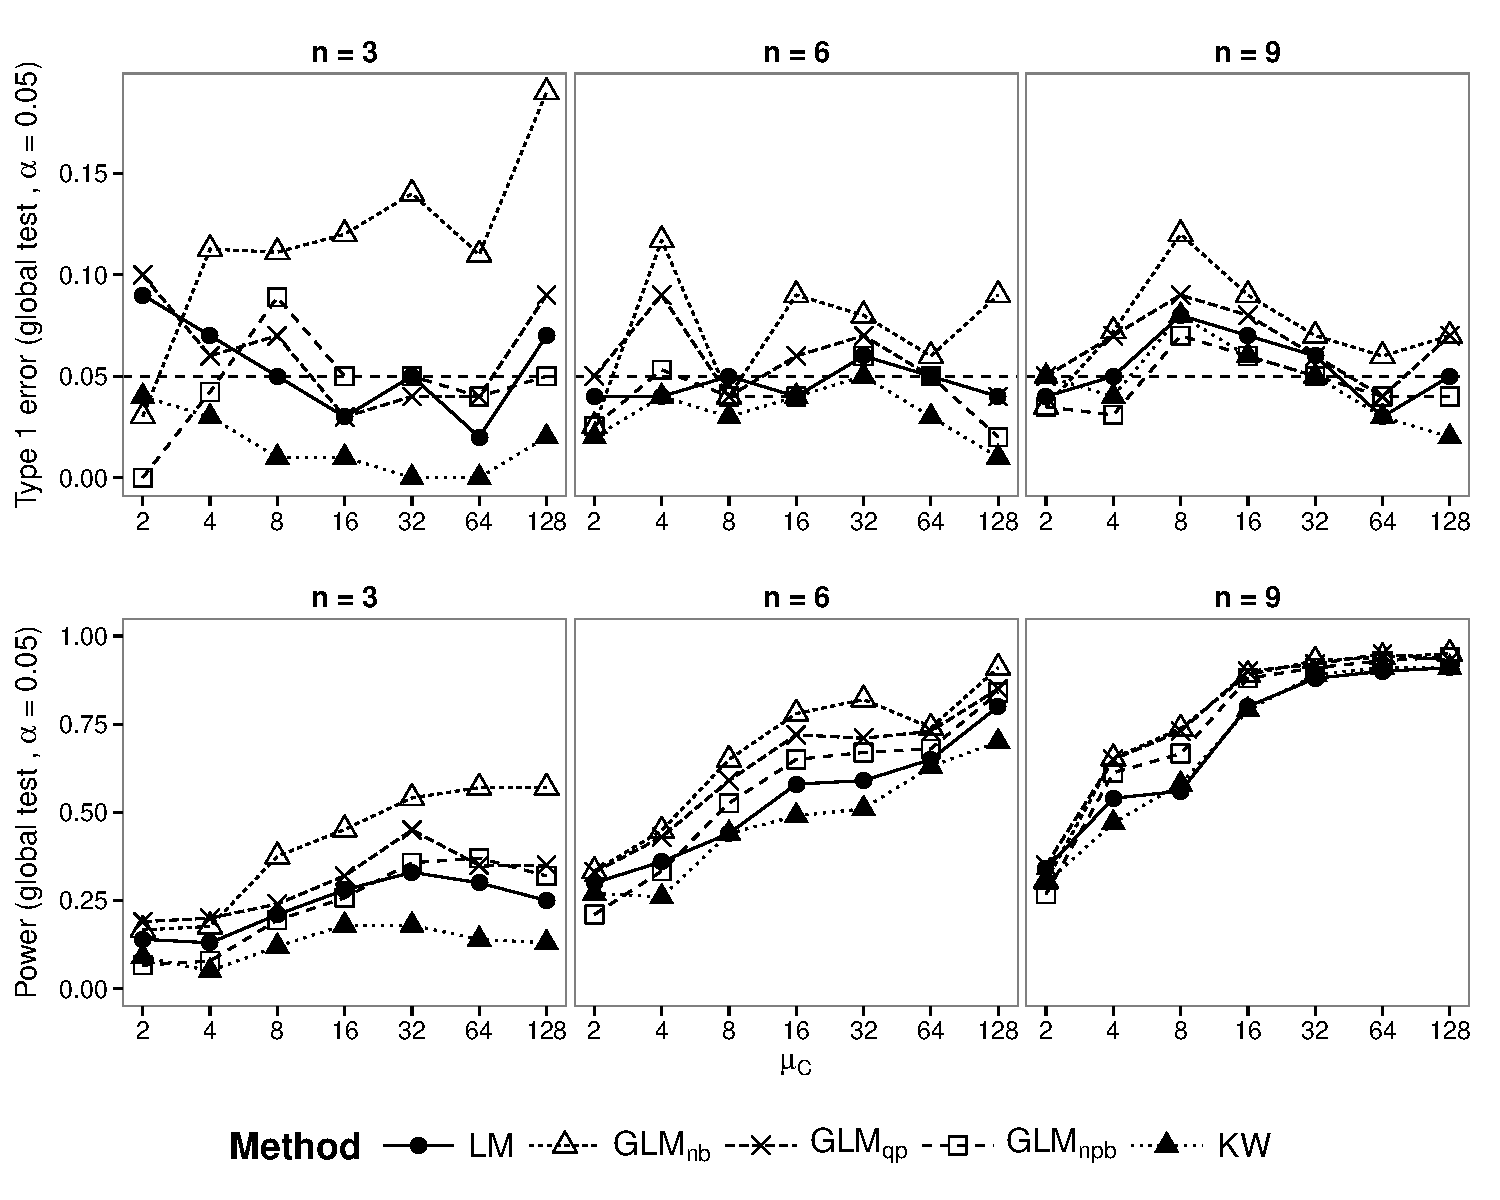
\includegraphics[width = 126mm]{p_glob_c.pdf}
  \caption{Count data simulations: Type 1 error (top) and Power (bottom) for the test of a treatment effect.
  Only type 1 errors \textless 25\% are displayed. 
  $GLM_p$ showed type 1 errors \textgreater 20\% in all simulation scenarios.
  Power levels for models with inflated type I error are shown for completeness.
  For n = \{3, 6\} and $\mu_C$ = \{2, 4\} less than 85\% of $GLM_{nb}$ and $GLM_{npb}$ models did converge.
  Dashed horizontal line denotes the nominal Type 1 error rate at $\alpha = 0.05$.
  }
  \label{fig:p_glob_c}
\end{figure*}

For LOEC determination $GLM_{nb}$ and $GLM_{p}$ showed an increased Type 1 error and all other methods were slightly conservative.
The inferences on LOEC generally showed less power.
$LM$ showed a mean reduction of 20.7\% and $GLM_{qp}$ of 24.3 \%.
Power to detect the LOEC was highest for $GLM_{qp}$. 
$LM$ and $WT$ showed less power, with $WT$ having no power to detect the LOEC at low sample sizes (Figure \ref{fig:p_loec_c}).

\begin{figure*}
  \centering
  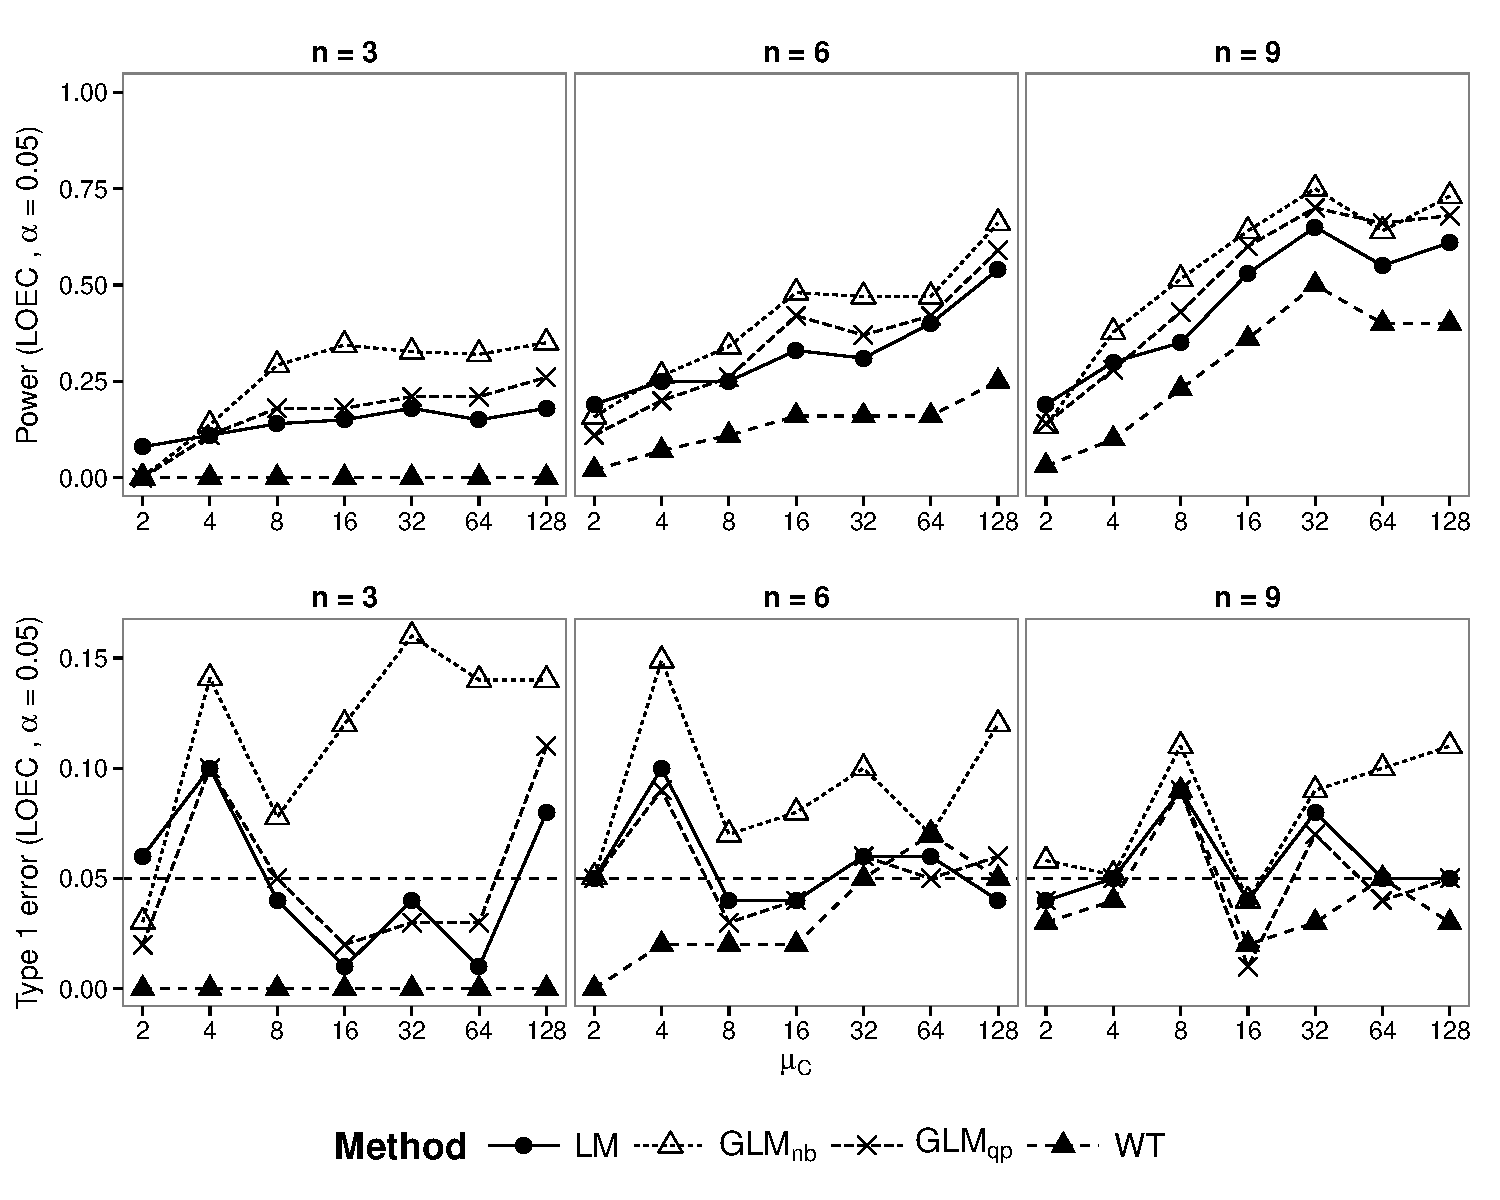
\includegraphics[width = 126mm]{p_loec_c.pdf}
  \caption{Count data simulations: Type 1 error (top) and Power (bottom) for determination of LOEC.
  For clarity only type 1 errors \textless 25\% are displayed.
  Power levels for models with inflated type I error are shown for completeness.
  For n = \{3, 6\} and $\mu_C$ = \{2, 4\} less than 85\% of $GLM_{nb}$ models did converge.
  Dashed horizontal line denotes the nominal Type 1 error rate at $\alpha = 0.05$.
  }
  \label{fig:p_loec_c}
\end{figure*}


\subsubsection{Binomial data}

$GLM_{bin}$ showed slightly increased type 1 error rates at low sample sizes and small effect sizes.
$KW$ was more conservative than $LM$ and $GLM_{bin}$.
In addition, $GLM_{bin}$ exhibited the greatest power for testing the treatment effect. 
This was especially apparent at low sample sizes (n = 3), with up to 27\% higher power compared to LM.
However, the differences between methods quickly vanished with increasing samples sizes (Figure \ref{fig:p_glob_p}).

\begin{figure*}
  \centering
  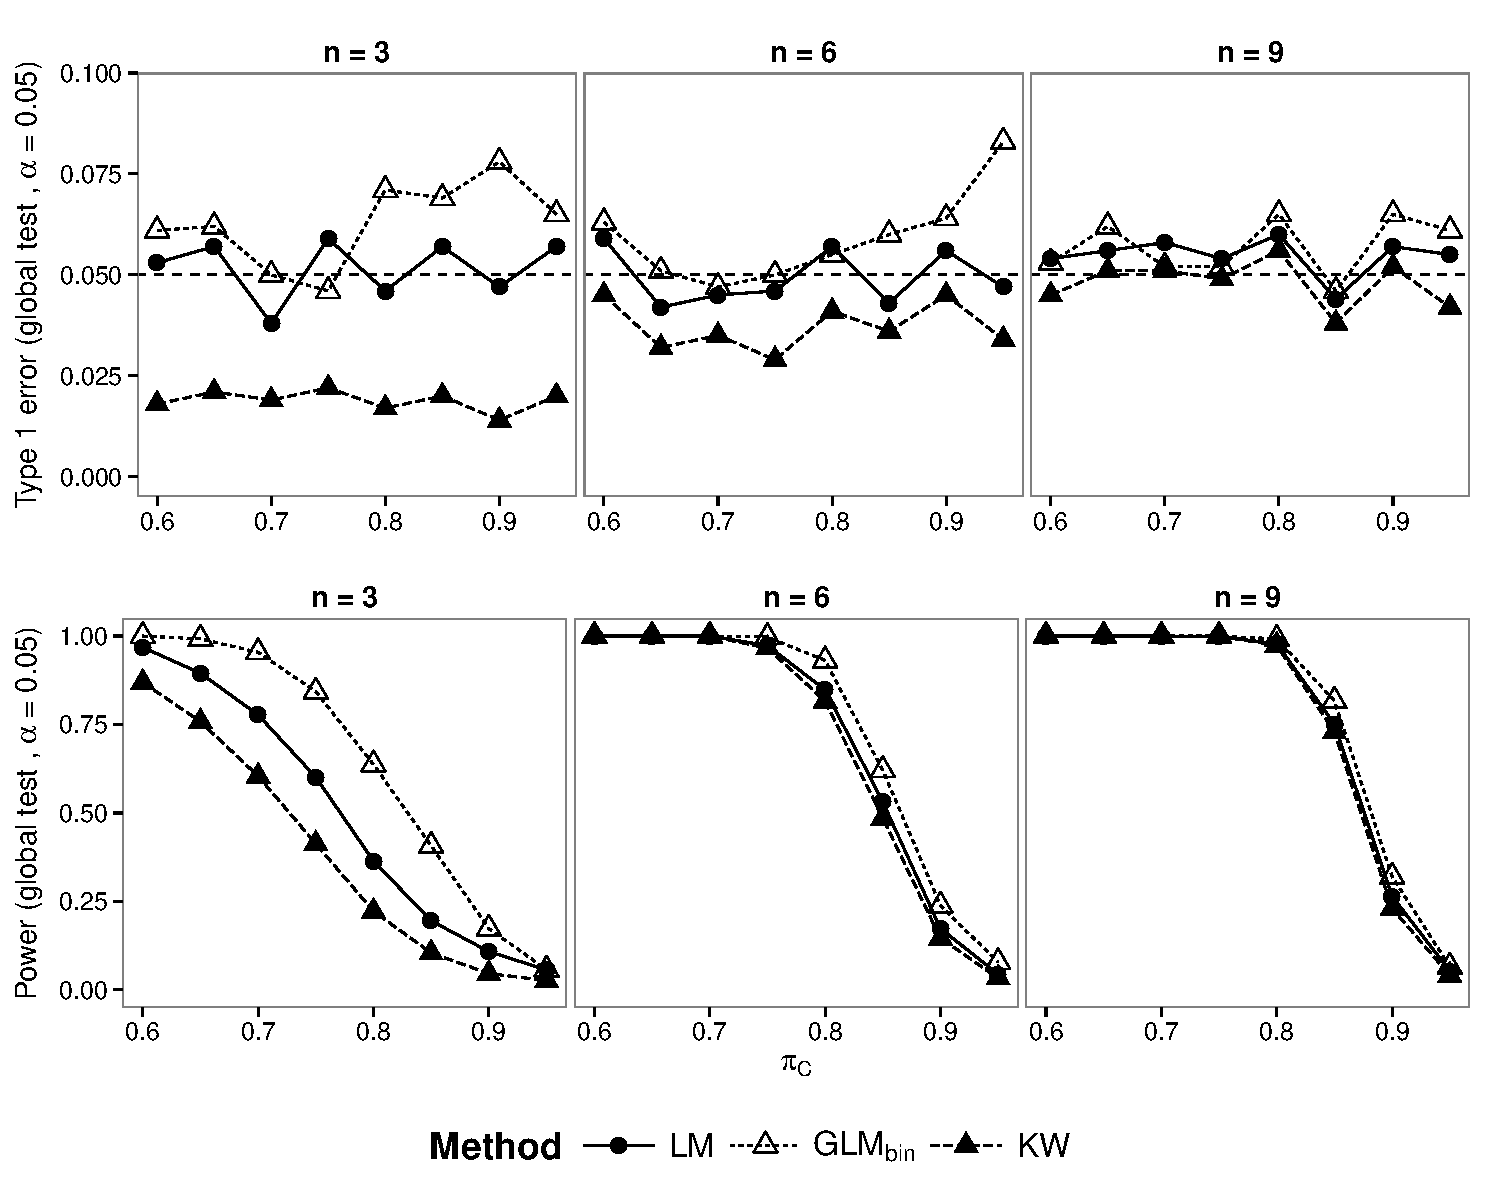
\includegraphics[width = 126mm]{p_glob_p.pdf}
  \caption{
  Binomial data simulations: 
  Type 1 error (top) and  power (bottom) for the test of a treatment effect. 
  Dashed horizontal line denotes the nominal Type 1 error rate at $\alpha = 0.05$.
  }
  \label{fig:p_glob_p}
\end{figure*}

For inference on LOEC we found that all methods were slightly conservative.
$WT$ was generally more conservative and $GLM_{bin}$ especially at low effect sizes ($p_E > 0.7$).
Inference on LOEC was not as powerful as inference on the general treatment effect.
Contrary to the general treatment effect, $LM$ showed the higher power than $GLM_{bin}$ at small sample sizes (n = {3, 6}).
$WT$ had no power for n = 3 and showed less power in the other simulation runs (Figure \ref{fig:p_loec_p}).

\begin{figure*}
  \centering
  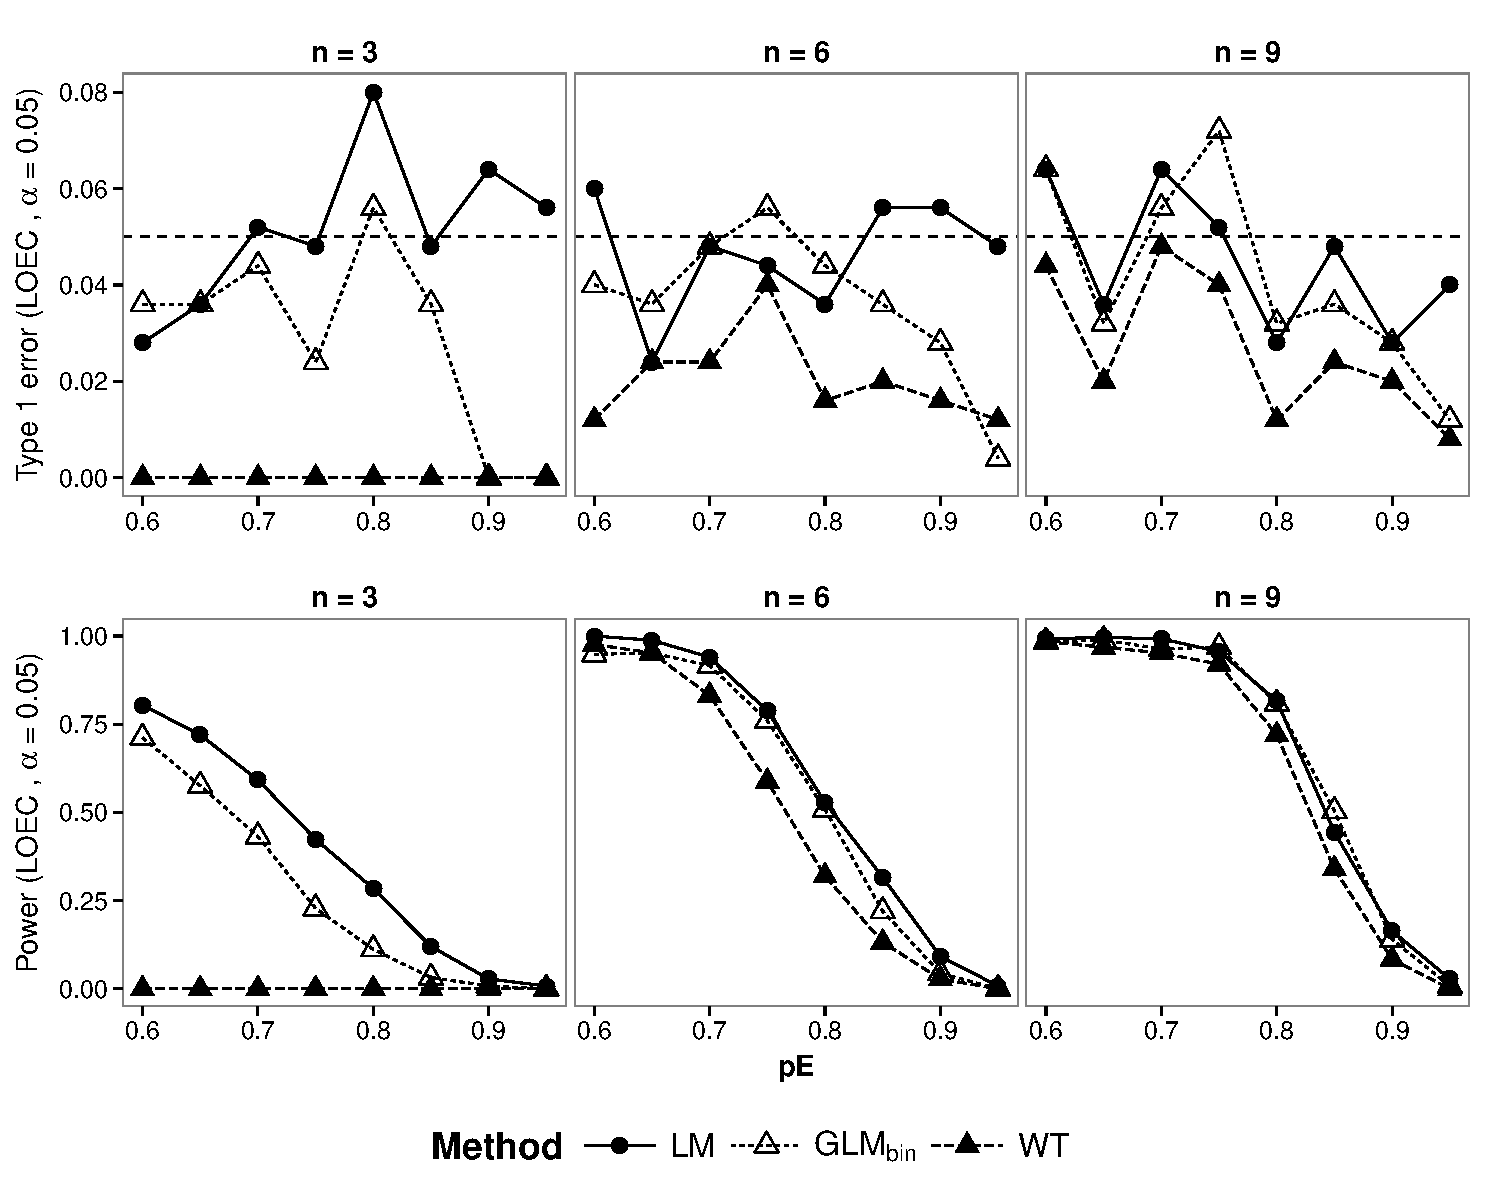
\includegraphics[width = 126mm]{p_loec_p.pdf}
  \caption{
  Binomial data simulations: 
  Type 1 error (top) and power (bottom) for the test for determination of LOEC. 
  Dashed horizontal line denotes the nominal Type 1 error rate at $\alpha = 0.05$.
  }
  \label{fig:p_loec_p}
\end{figure*}


%% ----------------------------------------------------------------------------
\section{Discussion}
\label{sec:disc}
\subsection{Case study}
%% ---- Case study
The outlined case study demonstrates that the choice of the statistical model and procedure can have substantial impact on ecotoxicological inferences and endpoints like the LOEC.
Therefore, ecotoxicologists should not base their inferences solely on statistical significance tests, but also on parameter estimates, their uncertainty and importance \citep{gelman_difference_2006}.
Nevertheless, \citet{ohara_not_2010} showed that $LM$ using a log transformation gave unreliable and biased parameter estimates, whereas GLMs performed well with little bias.
Bias occurs also when back-transforming means to the original scale, which explains the lower predicted means by $LM$ in Figure \ref{fig:example} \citep{rothery_cautionary_1988} and should be corrected for \citep{newman_regression_1993}.

This is further highlighted by the fact that for the same model (linear model of transformed data), \citet{brock_minimum_2015} reported a 10-fold lower LOEC (\mbox{0.3 mg/L}) then found in our study (3 mg/L, Figure \ref{fig:example}).
The reasons are manifold: \citep{brock_minimum_2015} used a $log(2~y + 1)$ transformation, whereas we used a $log(A~y + 1)$ transformation, where A = 2 / 11 = 0.182 \citep{van_den_brink_impact_2000}.
However, this contributed only little to the differences.
A much bigger impact had the type of multiple comparison: \citet{brock_minimum_2015} used a one-sided Williams test \citep{williams_comparison_1972}, whereas we used one-sided comparisons to the control (Dunnett contrasts).
In contrast to the Williams test, Dunnett contrasts do not assume a monotonic dose-response relationship and allow individual comparisons between treatment groups and the control.
However, under monotonicity they have less power, which explains the differences \citep{jaki_statistical_2013}.
Both types of multiple comparisons are available as multiple contrast tests in a GLM framework.
Therefore, our comparison of methods should be independent from the choice of contrast, which is determined by assumptions and research questions. 
 

%% ---- Guide GLMs
Overdispersion is common for ecological datasets \citep{warton_many_2005} and the case study illustrates the potential effects of overdispersion that is not accounted for: standard errors will be underestimated and significance overestimated (Figures \ref{fig:example}).
This is also shown by our simulations (Figures \ref{fig:p_glob_c}, \ref{fig:p_loec_c}) where $GLM_p$ showed increased type 1 error rates because of overdispersed simulated data. 
However, in factorial designs the mean-variance relationship can be easily checked by plotting mean versus variance of the treatment groups (see Supplement 2).
In the introduction we pointed out that there is little advice how to choose between the plenty of possible transformations - how do GLMs simplify this problem?
The distribution modelled can be chosen using knowledge about the data (e.g. bounds, integer or continuous data etc).
Knowing what type of data is modelled (see Methods section), the model selection process can be completely guided by the data and diagnostic tools. Therefore, choosing an appropriate model is easier than choosing between possible transformations.


\subsection{Simulations}
%% --- general low power
Our simulations showed that generally GLMs have greater power than data transformations.
However, the simulations also suggest that the power at the population level in common mesocosm experiments is low.
For common samples sizes ($n \le 4$ ) and a reduction in abundance of 50\% we found a low power to detect any treatment-related effect (\textless 50\% for methods with appropriate Type 1 error, Figure \ref{fig:p_glob_c}).
Statistical power to detect the correct LOEC was even lower (less than 25\%), which can be attributed to multiple testing.
The low power of all methods to detect significant treatment levels such as the LOEC or NOEC suggests that these endpoints from ecotoxicological studies should be interpreted with caution and underpins their criticism \citep{laskowski_good_1995,landis_well_2011}.

%% --- Multivariate + GLMM -------
Mesocosm studies allow also inferences on community level. 
For community analyses \emph{GLM for multivariate data} \citep{warton_distance-based_2012} have been proposed as alternative to Principal Response Curves (PRC) and yielded to similar inferences, but better indication of responsive taxa \citep{szocs_analysing_2015}. 
However, \citet{ter_braak_topics_2014} argue to use data transformations with community data because of their simplicity and robustness.
Although our simulations covered only simple experimental designs at the population level, findings may also extend to more complex situations. 
Nested or repeated designs with non-normal data could be analysed using Generalised Linear Mixed Models (GLMM) and may have advantages with respect to power \citep{stroup_rethinking_2014}.

%% --- Alternatives -------
To counteract the problems with low power at the population level \citet{brock_minimum_2015} proposed to take the Minimum Detectable Difference (MDD), a method to assess statistical power \emph{a posteriori}, for inference into account.
However, \emph{a priori} power analyses can be performed easily using simulations, even for complex experimental designs \citep{johnson_power_2014}, and might help to design, interpret and evaluate ecotoxicological studies.
Moreover, \citet{brock_minimum_2015} proposed that statistical power of mesocosm experiments can be increased by reducing sampling variability through improved sampling techniques and quantification methods, though they also caution against depleting populations through more exhaustive sampling.
As we showed, using appropriate statistical methods (like GLMs) can enhance the power at no extra costs.

%% --- Non-parametric
\citet{wang_making_2011} advocated that in the typical case of small sample sizes (n \textless 20) and non-normal data, non-parametric tests perform better than parametric tests assuming normality.
In contrast, our results showed that the often applied $KW$ and $WT$ have less power compared to $LM$.
Moreover, $GLMs$ always performed better than non-parametric tests. 
Though more powerful non-parametric tests may be available \citep{konietschke_rank-based_2012}, these are focused on hypothesis testing and do not provide estimation of effect sizes.
Additionally to testing, GLMs allow the estimation and interpretation of effects that might not be statistically significant, but ecologically relevant.
Therefore, we advise using GLMs instead of non-parametric tests for non-normal data.

%% ---- Problems GLM
We found an increased Type-I error for $GLM_{nb}$ at low sample sizes.
However, it is well known that the LR statistic is not reliable at small sample sizes \citep{bolker_generalized_2009,wilks_large-sample_1938}.
Parametric bootstrap ($GLM_{npb}$) is a valuable alternative in such situations and maintains appropriate levels (Figure \ref{fig:p_glob_c}).
Moreover, at small sample sizes and low abundances a significant amount of negative binomial models did not converge.
We used an iterative algorithm to fit these models \citep{venables_modern_2002}and other methods assessing the likelihood directly may perform better.

$GLM_{qp}$ showed higher statistical power than $GLM_{npb}$ (Figure \ref{fig:p_glob_c}, bottom).
This could be explained by the simpler mean-variance relationship of $GLM_{qp}$ (eqn. \ref{eqn:quasi} and \ref{eqn:negbin}), because at small samples sizes, low abundances or few treatment groups it is difficult to determine the mean-variance relationship.

%% --- binomial data
Binomial data are often collected in lab trials, where increasing the sample size may be relatively easy to accomplish. 
We found notable differences in power to detect a treatment effect for all simulated sample sizes.
Similarly, \citet{warton_arcsine_2011} also found that GLMs have higher power than arcsine transformed linear models.
Though we did not simulate overdispersed binomial data, this should be checked and accounted for.
In such situations a GLMM may offer an appealing alternative \citep{warton_arcsine_2011}.
At low effect sizes $GLM_{bin}$ became conservative with increasing $\pi_C$, although this effect lessened as sample size increased (Figure \ref{fig:p_loec_p}). 
This is because $\pi$ approaches its boundary and is also known as the \emph{Hauck-Donner effect} \citep{hauck_walds_1977}. A LR-Test or parametric bootstrap may provide an alternative in such situations \citep{bolker_generalized_2009}.
This can also explain why $LM$ performed better for deriving LOECs at low sample sizes.

GLMs can be fitted with several statistical software packages and many textbooks are available to introduce ecotoxicologists to these models (e.g. \citealt{zuur_beginners_2013} or \citealt{quinn_experimental_2009}).
We recommend that ecotoxicologists should change their models instead of their data.
GLMs should become a standard method in ecotoxicology and incorporated into respective guidelines.


\section{Compliance with Ethical Standards}
Conflict of Interest: The authors declare that they have no conflict of interest.

%% --------------------------------
\bibliography{references}
\bibliographystyle{spbasic}

\end{document}
